\documentclass[a4paper,12pt,titlepage]{article}
\usepackage{fancyhdr}
\usepackage{t1enc}
\usepackage[utf8]{inputenc}
\usepackage[magyar]{babel}
\usepackage{lmodern}
\usepackage[pdftex]{graphicx}
\usepackage[lflt]{floatflt}
\usepackage{epstopdf}
\usepackage{amsmath,amssymb}
\usepackage{icomma}
\usepackage{array}
\usepackage[unicode,colorlinks]{hyperref}
\usepackage{fullpage}
\usepackage{booktabs}
\usepackage{subcaption}
\usepackage{mathtools}
\usepackage{physics}

\hypersetup{allcolors=black}
\hypersetup{pdfstartview=FitH}
\hypersetup{pdfinfo={
	Title={Szupravezetőbeli spin- és töltéskorrelációk elméleti vizsgálata},
	Author={},
	Subject={},
	Keywords={}
}}


\title{\bf Szupravezetőbeli spin- és töltéskorrelációk elméleti vizsgálata}
\author{Hajdú Csanád \\ \small Témavezető: Dr.\ Zaránd Gergely Attila}
\date{2021.\ 05.\ 21.}
\topmargin = 0pt
\headheight = 14.5pt
\headsep = 14.5pt

\pagestyle{fancy}
\lhead{\small {{Szupravezetőbeli spin- és töltéskorrelációk elméleti vizsgálata} -- 2021.\ 05.\ 21.}}
\rhead{Hajdú Csanád}

\widowpenalty=10000 \clubpenalty=10000

% taken from https://tex.stackexchange.com/a/175245
\makeatletter
\DeclareRobustCommand*\uell{\mathpalette\@uell\relax}
\newcommand*\@uell[2]{
	% We need to adjust the width of \uell to be the same as \ell
	\setbox0=\hbox{$#1\ell$}
	\setbox1=\hbox{\rotatebox{10}{$#1\ell$}}
	\dimen0=\wd0 \advance\dimen0 by -\wd1 \divide\dimen0 by 2
	\mathord{\lower 0.1ex \hbox{\kern\dimen0\unhbox1\kern\dimen0}}
}

\newcommand{\KK}{{\vb*{k}}}
\newcommand{\LL}{{\vb*{\ell}}}
\newcommand{\RR}{{\vb*{r}}}
\newcommand{\phantomdagger}{{\phantom{\dagger}}}

\begin{document}

\maketitle

\tableofcontents \newpage


% ================================================================
\section{Bevezetés}

A szupravezetés a 20.\ század elején lett felfedezve Heike Kamerlingh Onnes holland fizikus által, amikor a higany ellenállását vizsgálta alacsony hőmérsékleten.  Azt tapasztalta, hogy $4,2$\,K alatt az ellenállás ugrásszerűen nullára csökkent.  Azóta sok más elemi fémnél és ötvözetnél is tapasztaltak szupravezetést, mindegyiknél van egy $T_\text{c}$ kritikus hőmérséklet, ami alatt a vezető disszipáció nélkül képes áramot vezetni.  A kritikus hőmérséklet értéke jellemzően $10$\,K alatt van, viszont vannak olyan anyagok is, amik már $100$\,K körül is szupravezetnek, az ilyen anyagokat magas hőmérsékletű szupravezetőknek nevezzük.  Az ilyen anyagok nagy előnye, hogy folyékony hélium helyett folyékony nitrogénnel is lehűthetők annyira, hogy szupravezessenek.

\begin{figure}[h!]
	\centering
	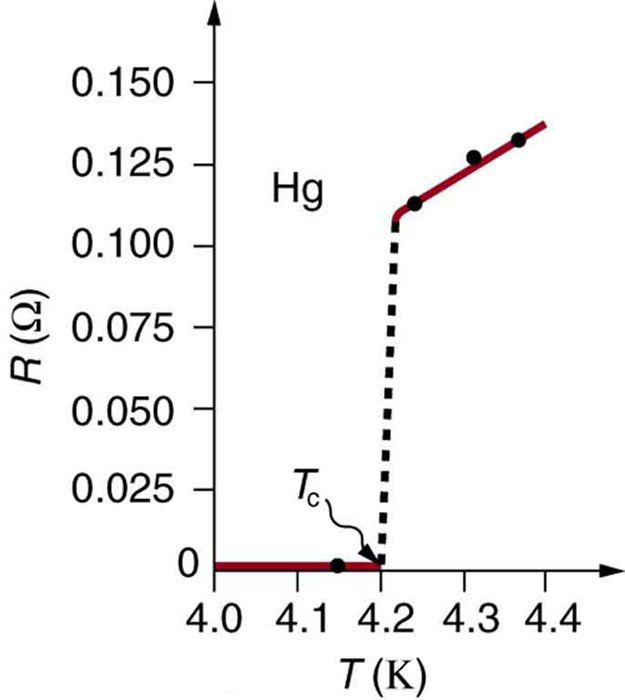
\includegraphics[width=5cm]{higany_R-vs-T.jpg}
	\caption[]{Egy higany minta ellenállása $T_\text{c}$ körül.\footnotemark}
\end{figure}
\footnotetext{\href{https://pressbooks.bccampus.ca/collegephysics/chapter/resistance-and-resistivity/}{\texttt{https://pressbooks.bccampus.ca/collegephysics/chapter/resistance-and-resistivity/}}}

A szupravezetés jelenségének fontos tulajdonsága a Meissner-effektus, ami egy minta belsejében a mágneses tér teljes kiszorítását jelenti.  Az ideális vezetésből következik, hogy a szupravezető minta belsejében a mágneses tér erőssége állandó, a Meissner-effektus viszont ennél nagyobb megszorítást tesz, azt hogy a minta belsejében a mágneses tér állandó és zérus.

A szupravezetőket széles körben használják fel, az egyik alapvető jelenség, amit kihasználnak a Josephson-effektus, ahol két szupravezető rész közé egy vékony szigetelőt tesznek be és a két vezetőre egy egyenfeszültséget kötnek.  Ezután azt tapasztaljuk, hogy a mintán egy váltóáram mérhető, aminek a frekvenciája arányos a vezetőkre kapcsolt feszültséggel.  A Josephson-effektust használja ki például az úgynevezett SQUID (superconducting quantum interference device), amivel mágneses tereket lehet nagy pontossággal mérni.  Ezen kívül még a Josephson-effektus alapján van definiálva az SI rendszerben a volt egysége.  Még fontos felhasználási terület a nagyterű szupravezető mágnesek, amiket többek között az orvostudományban is használnak MRI-kben.  Kvantumszámítógépekben is előnyös szupravezetőket használni a kvantumbitekhez, mivel az energiaspektrumukban van egy rés, így viszonylag magas hőmérsékleten is kicsi a zajuk.

A felfedezése óta számos elmélet született a szupravezetés jelenségének leírására, a két meghatározó elmélet a Ginzburg--Landau-elmélet, ami egy fenomenológikus elmélet, illetve a BCS-elmélet, ami egy mikroszkópikus leírást ad.
A Ginzburg--Landau-elméletet 1950-ben dolgozták ki Vitaly Ginzburg\footnote{Vitaly Lazarevich Ginzburg, Nobel-díjas (2003) orosz fizikus} és Lev Landau\footnote{Lev Davidovich Landau, Nobel-díjas (1962) orosz fizikus} orosz fizikusok, az elmélet jó leírást ad a szupravezetők makroszkópikus tulajdonságaira, még az olyan anyagoknál is, amikre a BCS-elmélet nem érvényes.  Ilyenek például a magas hőmérsékletű szupravezetők és nehéz fermion rendszerek.  Az elméletből ezen kívül következik még az első- és másodfajú szupravezetők megkülönböztetése.

A BCS-elméletet John Bardeen\footnote{John Bardeen, kétszeres Nobel-díjas (1956 és 1972) amerikai mérnök és fizikus}, Leon N.\ Cooper\footnote{Leon N.\ Cooper, Nobel-díjas (1972) amerikai fizikus} és John Robert Schrieffer\footnote{John Robert Schrieffer, Nobel-díjas (1972) amerikai fizikus} amerikai fizikusok dolgozták ki, és publikálták 1957-ben, az elmélet egy mikroszkópikus leírásmódot ad a szupravezetés jelenségére.  Az elmélet szerint a vezetési elektronok úgynevezett Cooper-párokat alkotnak egy köztük lévő vonzó kölcsönhatás miatt.  Ezt először Cooper mutatta meg, hogy akármilyen gyenge vonzó kölcsönhatás mellett is a normálállapot instabil lesz és az elektronok párokba rendeződnek.  A vonzó kölcsönhatás elektron-fonon kölcsönhatásokból származik és alacsony hőmérsékleten jön elő.  Az elektronok párokba rendeződését mérésekkel is igazolni lehet, azt tapasztaljuk, hogy a vezető részecskék töltése kétszerese az elektron töltésének.

Szupravezetésnél a minta energiaspektrumában megjelenik egy rés, ez az úgynevezett \emph{szupravezető gap}.  Ez a gap a hőmérséklet csökkenésével nő és $0$\,K-nél éri el a maximumát.  Kialakulása fontos szerepet játszik a szupravezetésben, azt tapasztaljuk, hogy ha a gap-et eltüntetjük például egy erős mágneses térrel, akkor a minta már nem fog szupravezetni.  A szupravezető gap értékének hőmérsékletfüggését a \ref{sc-gap}.\ ábrán láthatjuk.

\begin{figure}[h!]
	\centering
	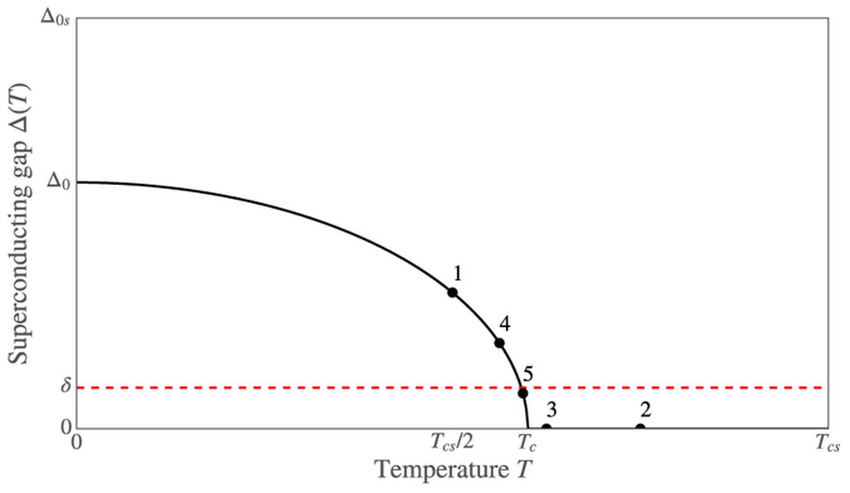
\includegraphics[width=12cm]{sc_gap.png}
	\caption[]{Szupravezető gap a hőmérséklet függvényében.\footnotemark}
	\label{sc-gap}
\end{figure}
\footnotetext{\href{https://www.researchgate.net/figure/Sketch-of-the-superconducting-gap-D-as-a-function-of-temperature-T-for-a-superconducting_fig3_305412985}{\texttt{https://www.researchgate.net/figure/Sketch-of-the-superconducting-gap-D-...}}}

A gap jelenléte azt is jelenti, hogy kevés gerjesztés van a szupravezető állapotban, tehát az elektronok többsége alapállapotban van.  Ez az állapot nagyon hasonlít a Bose--Einstein-kondenzációhoz, de a kialakulása másképp történik.

\newpage
A dolgozat célja az, hogy a szupravezető gap jelenléte mellett vizsgáljuk a spin- és töltéskorrelációs függvényeket, és összehasonlítsuk őket a normálállapotban lévő függvényekkel.  Hosszabb távon cél, hogy megértsük egy szupravezetőbe helyezett mágneses szennyezés körül kialakult úgynevezett Kondo-felhőben a spin-korrelációkat.

A dolgozatban először megnézzük a BCS Hamilton-operátor alakját, majd megmutatjuk, hogy ez transzformálható egy olyan alakra, ahol léptetőoperátorok jelennek meg.  Majd ezekkel a léptetőoperátorokkal felírjuk a korrelációs függvényeket.  Azt fogjuk látni, hogy ezekben két független függvény jelenik meg, amiket kiszámolunk mind normálállapotban, mind szupravezető állapotban.  Ezen függvények asszimpototikus viselkedését is megvizsgáljuk és analitikus közelítőfüggvényeket adunk meg közel- és távoltérben.  Végül ezek segítségével megkapjuk a spin- és töltéskorrelációs függvényeket normál- és szupravezető állapotban.

A számolásokhoz alapvető kvantumtérelméleti eszközöket használunk, részecske keltő és eltüntető operátorokat, illetve átlagtér közelítést.  Ezen kívül a BCS-elmélet közelítéseivel is élünk.



% ================================================================
\section{Fizikai modell}

\subsection{A BCS Hamilton-operátor}

A BCS-emélet egy egyszerű átlagtér modellt vesz a szupravezetők leírására.  A Hamilton-operátort két részből építi fel, a $H_0$ kinetikus és a $H_\text{int}$ kölcsönhatási tagokból.  A kinetikus tag
\begin{equation}
	H_0 = \sum\limits_\KK \xi_\KK \left( c_{\KK \uparrow}^\dagger c_{\KK \uparrow} + c_{\KK \downarrow}^\dagger c_{\KK \downarrow} \right),
\end{equation}
ahol $c_{\KK \sigma}^\dagger$ a $\left( \KK \sigma \right)$ sajátállapotú elektron keltő operátora és
$$ \xi_\KK = \frac{\hbar^2 k^2}{2 m} - E_\text{F} $$
az elektron kinetikus energiája a Fermi-energiához viszonyítva.

A kölcsönhatási tagnál azt a közelítést vesszük, hogy az elektronok csak a Cooper-párokon belül hatnak kölcsön.  Így $H_\text{int}$ felírható úgy, mint a Cooper-párok $\left( \KK \uparrow, -\KK \downarrow \right)$ állapotból $\left( \LL \uparrow, -\LL \downarrow \right)$ állapotba való átmenete,
\begin{equation} \label{H-int-def}
	H_\text{int} = \sum\limits_{\KK, \LL} V_{\KK \LL} \, c_{\LL \uparrow}^\dagger c_{-\LL \downarrow}^\dagger c_{-\KK \downarrow} c_{\KK \uparrow},
\end{equation}
ahol $V_{\KK \LL}$ az átmenet valószínűségi amplitúdója.  A BCS-elméletben ezt a valószínűséget úgy választjuk meg, hogy
$$ V_{\KK \LL} = \left\{ \begin{array}{rl}
	-V, & \text{ha } \left| \xi_\LL \right| < \hbar \omega_\text{D} \text{ és } \left| \xi_\KK \right| < \hbar \omega_\text{D} \\
	0, & \text{egyébként}
\end{array} \right. , $$
ahol $\omega_\text{D}$ a Debeye-frekvencia.  Ez azt jelenti, hogy csak a Fermi-felület közelében lévő elektronok hatnak kölcsön, tehát csak ezek lesznek vezető elektronok.

A kölcsönhatási tag alakjának meghatározásához vezessünk be egy variációs hullámyfüggvényt,
\begin{equation} \label{phi-tilde}
	\ket{\tilde{\phi}} \equiv \prod\limits_\KK \left( u_\KK + v_\KK \, c_{\KK \uparrow}^\dagger c_{-\KK \downarrow}^\dagger \right) \ket{0},
\end{equation}
ahol a $\ket{0}$ vákuum állapotba helyezünk be Cooper-párokat valamilyen amplitúdóval.  Az $u_\KK$ és $v_\KK$ együtthatók általános esetben komplexek és ahhoz, hogy $\ket{\tilde{\phi}}$ normálva legyen teljesülnie kell az
\begin{equation} \label{u-v-norm}
	\left| u_\KK \right|^2 + \left| v_\KK \right|^2 = 1
\end{equation}
relációnak.

Ezzel a formalizmussal a normálállapot hullámfüggvényét is felírhatjuk, ahol minden elektronállapot be van töltve a Fermi-felületig,
\begin{equation}
	\ket{\tilde{\phi}_\text{n}} = \prod\limits_{\left| \KK \right| < k_\text{F}} c_{\KK \uparrow}^\dagger c_{-\KK \downarrow}^\dagger \ket{0},
\end{equation}
ez az
\begin{equation}
	u_\KK = \left\{ \begin{array}{ll} 0, & \text{ha } \left| \KK \right| < k_\text{F} \\ 1, & \text{ha } \left| \KK \right| > k_\text{F} \end{array} \right.
	~~~ \text{és} ~~~
	v_\KK = \left\{ \begin{array}{ll} 1, & \text{ha } \left| \KK \right| < k_\text{F} \\ 0, & \text{ha } \left| \KK \right| > k_\text{F} \end{array} \right.
\end{equation}
együtthatóknak felel meg.

Vezessük be a $\Delta_\KK$ mennyiséget,
\begin{equation}
	\Delta_\KK^* \equiv \left\{ \begin{array}{ll}
	V \, {\sum\limits_\LL}^\prime \expval{c_{\LL \uparrow}^\dagger c_{-\LL \downarrow}^\dagger}, & \text{ha } \left| \xi_\KK \right| < \hbar \omega_\text{D} \\
	0, & \text{egyébként}
	\end{array} \right. ,
\end{equation}
ahol ${\sum_\LL}^\prime$ azt jelenti, hogy az összegzés csak a $\left| \xi_\LL \right| < \hbar \omega_\text{D}$ állapotokra van.  Ezután egy átlagtér közelítést alkalmazva a \eqref{H-int-def} definícióra azt kapjuk, hogy
\begin{equation}
	H_\text{int} = - \sum\limits_\KK \left( \Delta_\KK c_{\KK \uparrow}^\dagger c_{-\KK \downarrow}^\dagger + \Delta_\KK^* c_{-\KK \downarrow} c_{\KK \uparrow} \right) + \text{cst}.
\end{equation}

Ezzel felírhatjuk a teljes BCS Hamilton-operátort,
\begin{equation}
	H_\text{BCS} = H_0 + H_\text{int} = \sum\limits_\KK \left[ \xi_\KK \left( c_{\KK \uparrow}^\dagger c_{\KK \uparrow} + c_{\KK \downarrow}^\dagger c_{\KK \downarrow} \right) - \Delta_\KK c_{\KK \uparrow}^\dagger c_{-\KK \downarrow}^\dagger - \Delta_\KK^* c_{-\KK \downarrow} c_{\KK \uparrow} \right] + \text{cst}.
\end{equation}


\subsection{Az szupravezető-állapot léptetőoperátorai}

A BCS Hamilton-operátor spektrumának meghatározásához fejezzük ki azt léptetlőoperátorok segítségével,
\begin{equation} \label{H-BCS}
	H_\text{BCS} = \sum\limits_\KK E_\KK \left( \gamma_{\KK \uparrow}^\dagger \gamma_{\KK \uparrow} + \gamma_{\KK \downarrow}^\dagger \gamma_{\KK \downarrow} \right) + \text{cst},
\end{equation}
ahol a $\gamma_{\KK \sigma}$ operátorok a szupravezető-állapot kvázirészecskéinek léptetőoperátorai.  Továbbá igaz rájuk, hogy
\begin{equation} \label{gamma-anticommutator}
\begin{split}
	\anticommutator{\gamma_{\KK \sigma}^\phantomdagger}{\gamma_{\KK^\prime \sigma^\prime}^\phantomdagger} & = \anticommutator{\gamma_{\KK \sigma}^\dagger}{\gamma_{\KK^\prime \sigma^\prime}^\dagger} = 0, \\
	\anticommutator{\gamma_{\KK \sigma}^\phantomdagger}{\gamma_{\KK^\prime \sigma^\prime}^\dagger} & = \delta_{\KK \KK^\prime} \delta_{\sigma \sigma^\prime},
\end{split}
\end{equation}
ahol $\anticommutator{A}{B} = AB + BA$ az antikommutátor.  Ezen kívül kell lennie egy alapállapotnak is, amit a \eqref{phi-tilde} variációs hullámfüggvénynek veszünk.  Tudjuk, hogy a lefelé léptető operátornak ezt az állapotot a nullelembe kell vinnie, vagyis
\begin{equation} \label{gamma-zero}
	\gamma_{\KK \sigma} \ket{\tilde{\phi}} = \ket{}_0.
\end{equation}

Megmutatható, hogy a
\begin{equation} \label{gamma-def}
\begin{split}
	\gamma_{\KK \uparrow} & = u_\KK c_{\KK \uparrow} - v_\KK c_{-\KK \downarrow}^\dagger \\
	\gamma_{\KK \downarrow} & = u_\KK c_{\KK \downarrow} + v_\KK c_{-\KK \uparrow}^\dagger
\end{split}
\end{equation}
választásra teljesülnek a \eqref{gamma-anticommutator} és \eqref{gamma-zero} összefüggések.

A $\gamma_{\KK \sigma}$ operátorokra kapott kifejezést invertálva megkaphatjuk a $c_{\KK \sigma}$ operátorokat is,
\begin{equation}
\begin{split}
	c_{\KK \uparrow} & = u_\KK^* \gamma_{\KK \uparrow} + v_\KK \gamma_{-\KK \downarrow}^\dagger, \\
	c_{\KK \downarrow} & = u_\KK^* \gamma_{\KK \downarrow} - v_\KK \gamma_{-\KK \uparrow}^\dagger.
\end{split}
\end{equation}


\subsection{Az $u_\KK$ és $v_\KK$ együtthatók kiszámolása}

Az $u_\KK$ és $v_\KK$ együtthatók meghatározásához a léptetőoperátorok tulajdonságait használjuk fel, a \eqref{H-BCS} egyenletből következik, hogy
\begin{equation} \label{H-gamma-commutator}
	\commutator{H_\text{BCS}}{\gamma_{\KK \uparrow}^\dagger} = E_\KK \gamma_{\KK \uparrow}^\dagger.
\end{equation}
A $\commutator{H_\text{BCS}}{\gamma_{\KK \uparrow}^\dagger}$ kommutátor kiszámolásához használjuk fel a \eqref{gamma-def} összefüggést, tehát számoljuk ki egyenként $\commutator{H_\text{BCS}}{c_{\KK \uparrow}^\dagger}$ és $\commutator{H_\text{BCS}}{c_{-\KK \downarrow}}$ értékét.  A $c_{\KK \sigma}$ operátorok felcserélési relációjából könnyen belátható, hogy
\begin{equation}
	\commutator{H_\text{BCS}}{c_{\KK \uparrow}^\dagger} = \xi_\KK c_{\KK \uparrow}^\dagger - \Delta_\KK^* c_{-\KK \downarrow}
\end{equation}
és
\begin{equation}
	\commutator{H_\text{BCS}}{c_{-\KK \downarrow}} = -\xi_\KK c_{-\KK \downarrow} - \Delta_\KK c_{\KK \uparrow}^\dagger.
\end{equation}
Így a \eqref{H-gamma-commutator} összefüggés tovább írható,
\begin{equation}
	u_\KK^* \left( \xi_\KK c_{\KK \uparrow}^\dagger - \Delta_\KK^* c_{-\KK \downarrow} \right) - v_\KK^* \left( -\xi_\KK c_{-\KK \downarrow} - \Delta_\KK c_{\KK \uparrow}^\dagger \right) = E_\KK \left( u_\KK^* c_{\KK \uparrow}^\dagger - v_\KK^* c_{-\KK \downarrow} \right),
\end{equation}
amit egy lineáris egyenletrendszerként is felírhatunk,
\begin{equation}
	\begin{pmatrix}
		\xi_\KK & \Delta_\KK \\
		\Delta_\KK^* & -\xi_\KK
	\end{pmatrix} \begin{pmatrix} u_\KK^* \\ v_\KK^* \end{pmatrix}
	= E_\KK \begin{pmatrix} u_\KK^* \\ v_\KK^* \end{pmatrix}.
\end{equation}
A sajátértékekre $E_\KK = \pm \sqrt{\xi_\KK^2 + \left| \Delta_\KK \right|^2}$ adódik, amiből a pozitív előjelű feleltethető meg a felfelé léptető operátornak.  Végül az $u_\KK$ és $v_\KK$ együtthatókra, figyelembevéve a \eqref{u-v-norm} normálási feltételt,
\begin{equation}
	u_\KK = \frac{\Delta_\KK^*}{\sqrt{2 E_\KK \left( E_\KK - \xi_\KK \right)}} ~~~ \text{és} ~~~ v_\KK = \frac{E_\KK - \xi_\KK}{\sqrt{2 E_\KK \left( E_\KK - \xi_\KK \right)}}
\end{equation}
adódik.


\subsection{BCS közelítés és a mi közelítésünk}

A BCS-elméletben $\Delta_\LL$ definíciója
\begin{equation}
	\Delta_\LL = \left\{ \begin{array}{ll} \Delta, & \text{ha } \left| \xi_\LL \right| < \hbar \omega_\text{D} \\ 0, & \text{ha } \left| \xi_\LL \right| > \hbar \omega_\text{D} \end{array} \right. ,
\end{equation}
ahol $\omega_\text{D}$ a Debeye-frekvencia.  Ez azt jelenti, hogy csak a Fermi-felület közelében lévő elektronok vesznek részt a szupravezetésben.

A BCS-elméletben használt éles levágás helyett mi egy analitikus függvényt használunk, hogy a számolás során kapott integrálokat egyszerűbben tudjuk analitikusan kezelni.  A használt levágás
$$ \frac{1}{\left( \frac{\xi_\LL}{\hbar \omega_\text{D}} \right)^4 + 1} $$
alakú, ami az éles levágáshoz hasonlóan nagyjából a $\left[ -\hbar \omega_\text{D}, \hbar \omega_\text{D} \right]$ tartományon nem zérus, $\Delta_\LL$ értékét mi is konstansnak vesszük a vizsgált tartományon, $\Delta_\LL \equiv \Delta$.

A legtöbb szupravezetőben $\left|\Delta\right| \ll \hbar \omega_\text{D} \ll E_\text{F}$, amit a számolásaink során ki is fogunk használni.



% ================================================================
\section{Korrelátorok számolása}

Vezessük be a $\psi_\sigma(\RR)$ operátorokat, amik a $c_{\KK \sigma}$ operátorokhoz hasonlóan keltő operátorok, viszont egy $\left( \KK \sigma \right)$ sajátállapotú részecske helyett egy $\left( \RR \sigma \right)$ sajátállapotút rak be az állapotfüggvénybe.  A keltő operátorok transzformációja szerint kifejezhetjük őket egymással,
\begin{equation} \label{psi}
\begin{split}
	\psi_\uparrow(\RR) & = \frac{1}{\sqrt{V}} \sum\limits_\KK e^{i \KK \RR} c_{\KK \uparrow} = \frac{1}{\sqrt{V}} \sum\limits_\KK e^{i \KK \RR} \left( u_\KK^* \gamma_{\KK \uparrow} + v_\KK \gamma_{-\KK \downarrow}^\dagger \right), \\
	\psi_\uparrow^\dagger(\RR) & = \frac{1}{\sqrt{V}} \sum\limits_\KK e^{-i \KK \RR} c_{\KK \uparrow}^\dagger = \frac{1}{\sqrt{V}} \sum\limits_\KK e^{-i \KK \RR} \left( u_\KK \gamma_{\KK \uparrow}^\dagger + v_\KK^* \gamma_{-\KK \downarrow} \right), \\
	\psi_\downarrow(\RR) & = \frac{1}{\sqrt{V}} \sum\limits_\KK e^{-i \KK \RR} c_{-\KK \downarrow} = \frac{1}{\sqrt{V}} \sum\limits_\KK e^{-i \KK \RR} \left( -v_\KK \gamma_{\KK \uparrow}^\dagger + u_\KK^* \gamma_{-\KK \downarrow} \right), \\
	\psi_\downarrow^\dagger(\RR) & = \frac{1}{\sqrt{V}} \sum\limits_\KK e^{i \KK \RR} c_{-\KK \downarrow}^\dagger = \frac{1}{\sqrt{V}} \sum\limits_\KK e^{i \KK \RR} \left( -v_\KK^* \gamma_{\KK \uparrow} + u_\KK \gamma_{-\KK \downarrow}^\dagger \right).
\end{split}
\end{equation}


\subsection{Töltéskorreláció}

A \eqref{psi} keltő operátorokkal felírhatjuk a szupravezető állapotban a töltéskorrelációt,
\begin{equation}
	e^2 \left< \rho(\RR) \rho(\RR^\prime) \right> = e^2 \sum\limits_{\sigma, \sigma^\prime} \left< \psi_\sigma^\dagger(\RR) \psi_\sigma(\RR) \psi_{\sigma^\prime}^\dagger(\RR^\prime) \psi_{\sigma^\prime}(\RR^\prime) \right>,
\end{equation}
ahol a várhatóértékhez az $\left< A \right> = \matrixelement{\tilde{\phi}}{A}{\tilde{\phi}}$ jelölést használtuk.  Az összeg egyes tagjait kiszámolhatjuk \eqref{psi} segítségével.

Először írjuk fel $\left< \psi_\uparrow^\dagger(\RR) \psi_\uparrow(\RR) \psi_\uparrow^\dagger(\RR^\prime) \psi_\uparrow(\RR^\prime) \right>$-t,
\begin{multline}
	\left< \psi_\uparrow^\dagger(\RR) \psi_\uparrow(\RR) \psi_\uparrow^\dagger(\RR^\prime) \psi_\uparrow(\RR^\prime) \right> = \frac{1}{V^2} \sum\limits_{\substack{\KK_1, \KK_2, \\ \KK_3, \KK_4}} e^{-i \KK_1 \RR} e^{i \KK_2 \RR} e^{-i \KK_3 \RR^\prime} e^{i \KK_4 \RR^\prime} \cdot \\
	\cdot \left< \left( u_{\KK_1} \gamma_{\KK_1 \uparrow}^\dagger + v_{\KK_1}^* \gamma_{-\KK_1 \downarrow} \right) \left( u_{\KK_2}^* \gamma_{\KK_2 \uparrow} + v_{\KK_2} \gamma_{-\KK_2 \downarrow}^\dagger \right)
	\right. \\ \left.
	\left( u_{\KK_3} \gamma_{\KK_3 \uparrow}^\dagger + v_{\KK_3}^* \gamma_{-\KK_3 \downarrow} \right) \left( u_{\KK_4}^* \gamma_{\KK_4 \uparrow} + v_{\KK_4} \gamma_{-\KK_4 \downarrow}^\dagger \right) \right>.
\end{multline}
Kihasználhatjuk, hogy $\gamma_{\KK \sigma} \ket{\tilde{\phi}} = 0$ és $\bra{\tilde{\phi}} \gamma_{\KK \sigma}^\dagger = 0$, amivel
\begin{multline}
	\left< \psi_\uparrow^\dagger(\RR) \psi_\uparrow(\RR) \psi_\uparrow^\dagger(\RR^\prime) \psi_\uparrow(\RR^\prime) \right> = \frac{1}{V^2} \sum\limits_{\substack{\KK_1, \KK_2, \\ \KK_3, \KK_4}} e^{-i \KK_1 \RR} e^{i \KK_2 \RR} e^{-i \KK_3 \RR^\prime} e^{i \KK_4 \RR^\prime} \cdot \\
	\cdot \left( \left< v_{\KK_1}^* u_{\KK_2}^* u_{\KK_3} v_{\KK_4} \cdot \gamma_{-\KK_1 \downarrow} \gamma_{\KK_2 \uparrow} \gamma_{\KK_3 \uparrow}^\dagger \gamma_{-\KK_4 \downarrow}^\dagger \right> + \left< v_{\KK_1}^* v_{\KK_2} v_{\KK_3}^* v_{\KK_4} \cdot \gamma_{-\KK_1 \downarrow} \gamma_{-\KK_4 \downarrow}^\dagger \gamma_{-\KK_3 \downarrow} \gamma_{-\KK_4 \downarrow}^\dagger \right> \right)
\end{multline}
adódik.  Ezután felhasználhatjuk a \eqref{gamma-anticommutator} összefüggéseket, illetve azt, hogy
$$ \gamma_{\KK \sigma} \gamma_{\KK^\prime \sigma^\prime}^\dagger \ket{\tilde{\phi}} = \delta_{\KK \KK^\prime} \delta_{\sigma \sigma^\prime} \ket{\tilde{\phi}}. $$
Ezekkel a végső alak
\begin{multline}
	\left< \psi_\uparrow^\dagger(\RR) \psi_\uparrow(\RR) \psi_\uparrow^\dagger(\RR^\prime) \psi_\uparrow(\RR^\prime) \right> = \\
	= \left( \frac{1}{V} \sum\limits_\KK e^{-i \KK \left( \RR - \RR^\prime \right)} \left| v_\KK \right|^2 \right) \left( \frac{1}{V} \sum\limits_\KK e^{-i \KK \left( \RR - \RR^\prime \right)} \left| u_\KK \right|^2 \right) + \left( \frac{1}{V} \sum\limits_\KK \left| v_\KK \right|^2 \right)^2.
\end{multline}
A többi korrelátort is hasonlóan kiszámíthatjuk, azokra
\begin{multline}
	\left< \psi_\downarrow^\dagger(\RR) \psi_\downarrow(\RR) \psi_\downarrow^\dagger(\RR^\prime) \psi_\downarrow(\RR^\prime) \right> = \\
	= \left( \frac{1}{V} \sum\limits_\KK e^{-i \KK \left( \RR - \RR^\prime \right)} \left| v_\KK \right|^2 \right) \left( \frac{1}{V} \sum\limits_\KK e^{-i \KK \left( \RR - \RR^\prime \right)} \left| u_\KK \right|^2 \right) + \left( \frac{1}{V} \sum\limits_\KK \left| v_\KK \right|^2 \right)^2,
\end{multline}
\begin{multline}
	\left< \psi_\uparrow^\dagger(\RR) \psi_\uparrow(\RR) \psi_\downarrow^\dagger(\RR^\prime) \psi_\downarrow(\RR^\prime) \right> = \\
	= \left( \frac{1}{V} \sum\limits_\KK e^{-i \KK \left( \RR - \RR^\prime \right)} u_\KK v_\KK^* \right) \left( \frac{1}{V} \sum\limits_\KK e^{i \KK \left( \RR - \RR^\prime \right)} u_\KK^* v_\KK \right) + \left( \frac{1}{V} \sum\limits_\KK \left| v_\KK \right|^2 \right)^2,
\end{multline}
\begin{multline}
	\left< \psi_\downarrow^\dagger(\RR) \psi_\downarrow(\RR) \psi_\uparrow^\dagger(\RR^\prime) \psi_\uparrow(\RR^\prime) \right> = \\
	= \left( \frac{1}{V} \sum\limits_\KK e^{i \KK \left( \RR - \RR^\prime \right)} u_\KK v_\KK^* \right) \left( \frac{1}{V} \sum\limits_\KK e^{-i \KK \left( \RR - \RR^\prime \right)} u_\KK^* v_\KK \right) + \left( \frac{1}{V} \sum\limits_\KK \left| v_\KK \right|^2 \right)^2
\end{multline}
adódnak.

Az eredmények megértéséhez számoljuk ki a $\left< \psi_\sigma(\RR) \psi_{\sigma^\prime}(\RR^\prime) \right>$ alakú különféle korrelátorokat is, ezeket az előzőekhez hasonlóan tehetjük meg, végeredményül
\begin{equation}
\begin{split}
	G(\RR - \RR^\prime) \coloneqq & \left< \psi_\uparrow^\dagger(\RR) \psi_\uparrow^\phantomdagger(\RR^\prime) \right> = \frac{1}{V} \sum\limits_\KK e^{-i \KK \left( \RR - \RR^\prime \right)} \left| v_\KK \right|^2, \\
	& \left< \psi_\downarrow^\dagger(\RR) \psi_\downarrow^\phantomdagger(\RR^\prime) \right> = G(\RR - \RR^\prime), \\
	& \left< \psi_\uparrow^\phantomdagger(\RR) \psi_\uparrow^\dagger(\RR^\prime) \right> = \delta(\RR - \RR^\prime) - G(\RR - \RR^\prime), \\
	& \left< \psi_\downarrow^\phantomdagger(\RR) \psi_\downarrow^\dagger(\RR^\prime) \right> = \delta(\RR - \RR^\prime) - G(\RR - \RR^\prime), \\
	F(\RR - \RR^\prime) \coloneqq & \left< \psi_\uparrow^\dagger(\RR) \psi_\downarrow^\dagger(\RR^\prime) \right> = \frac{1}{V} \sum\limits_\KK e^{-i \KK \left( \RR - \RR^\prime \right)} u_\KK v_\KK^*, \\
	& \left< \psi_\downarrow^\dagger(\RR) \psi_\uparrow^\dagger(\RR^\prime) \right> = -F(\RR - \RR^\prime), \\
	& \left< \psi_\uparrow^\phantomdagger(\RR) \psi_\downarrow^\phantomdagger(\RR^\prime) \right> = -F^*(\RR - \RR^\prime), \\
	& \left< \psi_\downarrow^\phantomdagger(\RR) \psi_\uparrow^\phantomdagger(\RR^\prime) \right> = F^*(\RR - \RR^\prime), \\
\end{split}
\end{equation}
adódnak, ahol bevezettük az $F(\RR)$ és $G(\RR)$ függvényeket.  A nem felírt korrelátorok mind nullák.  Ezekkel kifejezve a korábbi eredményeket,
\begin{equation}
\begin{split} \label{density-components}
	\left< \psi_\uparrow^\dagger(\RR) \psi_\uparrow(\RR) \psi_\uparrow^\dagger(\RR^\prime) \psi_\uparrow(\RR^\prime) \right> & = \left< \psi_\uparrow^\dagger(\RR) \psi_\uparrow(\RR^\prime) \right> \left< \psi_\uparrow(\RR) \psi_\uparrow^\dagger(\RR^\prime) \right> + \left< \psi_\uparrow^\dagger(\RR) \psi_\uparrow(\RR) \right> \left< \psi_\uparrow^\dagger(\RR^\prime) \psi_\uparrow(\RR^\prime) \right>,  \\
	\left< \psi_\downarrow^\dagger(\RR) \psi_\downarrow(\RR) \psi_\downarrow^\dagger(\RR^\prime) \psi_\downarrow(\RR^\prime) \right> & = \left< \psi_\downarrow^\dagger(\RR) \psi_\downarrow(\RR^\prime) \right> \left< \psi_\downarrow(\RR) \psi_\downarrow^\dagger(\RR^\prime) \right> + \left< \psi_\downarrow^\dagger(\RR) \psi_\downarrow(\RR) \right> \left< \psi_\downarrow^\dagger(\RR^\prime) \psi_\downarrow(\RR^\prime) \right>,  \\
	\left< \psi_\uparrow^\dagger(\RR) \psi_\uparrow(\RR) \psi_\downarrow^\dagger(\RR^\prime) \psi_\downarrow(\RR^\prime) \right> & = -\left< \psi_\uparrow^\dagger(\RR) \psi_\downarrow^\dagger(\RR^\prime) \right> \left< \psi_\uparrow(\RR) \psi_\downarrow(\RR^\prime) \right> + \left< \psi_\uparrow^\dagger(\RR) \psi_\uparrow(\RR) \right> \left< \psi_\downarrow^\dagger(\RR^\prime) \psi_\downarrow(\RR^\prime) \right>,  \\
	\left< \psi_\downarrow^\dagger(\RR) \psi_\downarrow(\RR) \psi_\uparrow^\dagger(\RR^\prime) \psi_\uparrow(\RR^\prime) \right> & = -\left< \psi_\downarrow^\dagger(\RR) \psi_\uparrow^\dagger(\RR^\prime) \right> \left< \psi_\downarrow(\RR) \psi_\uparrow(\RR^\prime) \right> + \left< \psi_\downarrow^\dagger(\RR) \psi_\downarrow(\RR) \right> \left< \psi_\uparrow^\dagger(\RR^\prime) \psi_\uparrow(\RR^\prime) \right>,
\end{split}
\end{equation}
az $F(\RR)$ és $G(\RR)$ függvényekkel kifejezve
\begin{equation} \label{correlators-F-G}
\begin{split}
	\left< \psi_\uparrow^\dagger(\RR) \psi_\uparrow(\RR) \psi_\uparrow^\dagger(\RR^\prime) \psi_\uparrow(\RR^\prime) \right> & = G(\RR - \RR^\prime) \cdot \left( \delta(\RR - \RR^\prime) - G(\RR - \RR^\prime) \right) + G^2(0), \\
	\left< \psi_\downarrow^\dagger(\RR) \psi_\downarrow(\RR) \psi_\downarrow^\dagger(\RR^\prime) \psi_\downarrow(\RR^\prime) \right> & = G(\RR - \RR^\prime) \cdot \left( \delta(\RR - \RR^\prime) - G(\RR - \RR^\prime) \right) + G^2(0), \\
	\left< \psi_\uparrow^\dagger(\RR) \psi_\uparrow(\RR) \psi_\downarrow^\dagger(\RR^\prime) \psi_\downarrow(\RR^\prime) \right> & = \left| F(\RR - \RR^\prime) \right|^2 + G^2(0), \\
	\left< \psi_\downarrow^\dagger(\RR) \psi_\downarrow(\RR) \psi_\uparrow^\dagger(\RR^\prime) \psi_\uparrow(\RR^\prime) \right> & = \left| F(\RR - \RR^\prime) \right|^2 + G^2(0).
\end{split}
\end{equation}
A \eqref{density-components} összefüggésben felismerhetjük a Wick-tételt, ami szerint ki lehet bontani a várhatóértéket több egyszerűbb tag összegére.

A töltéskorrelációs függvényt így felírhatjuk az $F(\RR)$ és $G(\RR)$ függvények segítségével,
\begin{equation}
	e^2 \left< \rho(\RR) \rho(\RR^\prime) \right> = e^2 \left( 4 \, G^2(0) + 2 \left| F(\RR - \RR^\prime) \right|^2 - 2 \, G^2(\RR - \RR^\prime) + 2 \, G(0) \cdot \delta(\RR - \RR^\prime) \right).
\end{equation}


\subsection{Spinkorreláció}

A spinsűrűség operátorok felírhatók a \eqref{psi} keltő operátorok segítségével,
\begin{equation}
	s_\alpha(\RR) = \frac{\hbar}{2} \begin{pmatrix} \psi_\uparrow^\dagger(\RR) & \psi_\downarrow^\dagger(\RR) \end{pmatrix} \sigma_\alpha \begin{pmatrix} \psi_\uparrow(\RR) \\ \psi_\downarrow(\RR) \end{pmatrix},
\end{equation}
ahol $\alpha = x, y, z$ és $\sigma_\alpha$ a Pauli-mátrixok.  A teljes spinkorrelációs függvény
\begin{equation}
	\left< s(\RR) s(\RR^\prime) \right> = \sum_\alpha \left< s_\alpha(\RR) s_\alpha(\RR^\prime) \right>.
\end{equation}
A függvény kiszámolása hasonlóan tehető meg, mint a töltéskorrelációs függvénynél, először számoljuk ki $\left< s_z(\RR) s_z(\RR^\prime) \right>$ értékét.
\begin{multline}
	\left< s_z(\RR) s_z(\RR^\prime) \right> = \frac{\hbar^2}{4} \left( \left< \psi_\uparrow^\dagger(\RR) \psi_\uparrow(\RR) \psi_\uparrow^\dagger(\RR^\prime) \psi_\uparrow(\RR^\prime) \right> - \left< \psi_\uparrow^\dagger(\RR) \psi_\uparrow(\RR) \psi_\downarrow^\dagger(\RR^\prime) \psi_\downarrow(\RR^\prime) \right> -
	\right. \\ \left. -
	\left< \psi_\downarrow^\dagger(\RR) \psi_\downarrow(\RR) \psi_\uparrow^\dagger(\RR^\prime) \psi_\uparrow(\RR^\prime) \right> + \left< \psi_\downarrow^\dagger(\RR) \psi_\downarrow(\RR) \psi_\downarrow^\dagger(\RR^\prime) \psi_\downarrow(\RR^\prime) \right> \right),
\end{multline}
a \eqref{correlators-F-G} összefüggéseket felhasználva
\begin{equation}
	\left< s_z(\RR) s_z(\RR^\prime) \right> = \frac{\hbar^2}{2} \left( -\left| F(\RR - \RR^\prime) \right|^2 - G^2(\RR - \RR^\prime) + G(0) \cdot \delta(\RR - \RR^\prime) \right).
\end{equation}
$\left< s_x(\RR) s_x(\RR^\prime) \right>$ és $\left< s_y(\RR) s_y(\RR^\prime) \right>$-t kiszámolva azt látjuk, hogy a három korrelátor értéke megegyezik, így a teljes spinkorrelációs függvény
\begin{equation}
\begin{split}
	\left< s(\RR) s(\RR^\prime) \right> & = \frac{3 \hbar^2}{2} \left( -\left| F(\RR - \RR^\prime) \right|^2 - G^2(\RR - \RR^\prime) + G(0) \cdot \delta(\RR - \RR^\prime) \right) \\
	& = \frac{3 \hbar^2}{4} \left( \left< \rho(\RR) \rho(\RR^\prime) \right> - 4 \left| F(\RR - \RR^\prime) \right|^2 - 4 \, G^2(0) \right).
\end{split}
\end{equation}


% ================================================================
\section{$F(\RR)$ és $G(\RR)$ függvények meghatározása}

\subsection{Normálállapot}

\subsubsection{$F(\RR)$ normálállapotban}
\subsubsection{$G(\RR)$ normálállapotban}

\subsection{Szupravezető állapot járuléka}

\subsubsection{$F(\RR)$ szupravezető járuléka}
\subsubsection{$G(\RR)$ szupravezető járuléka}

\subsection{Asszimptotikus viselkedés}



% ================================================================
\section{Spin- és töltéskorrelációs függvények}

\subsection{Töltéskorreláció}
\subsection{Spinkorreláció}



\pdfbookmark{Hivatkozások}{bm:hivatkozasok}

\begin{thebibliography}{}
\end{thebibliography}


\end{document}
